\section{Solutions Last Week}
\begin{frame}[fragile,allowframebreaks]\frametitle{Exercises} 
  \begin{enumerate}
  \item use a t-test to compare \texttt{TTime} according to \texttt{Stim.Type}, visualize it. What is the problem?
  \item now do the same for Subject 1 on pre and post test (use \texttt{filter()} or indexing to get the resp. subsets)
  \item use the following code to do the test on every subset \texttt{Subject} and \texttt{testid}, try to figure what is happening in each step:\tiny
\begin{verbatim}
data.l <- split(data,list(data$Subject,data$testid),drop=T)
tmp.l <- lapply(data.l,function(x) {
    if(min(table(x$Stim.Type)) < 5) return(NULL)
    tob <- t.test(x$TTime ~ x$Stim.Type)
    tmp <- data.frame(
        Subject = unique(x$Subject),
        testid = unique(x$testid),
        mean.group.1 = tob$estimate[1],
        mean.group.2 = tob$estimate[2],
        name.test.stat = tob$statistic,
        conf.lower = tob$conf.int[1],
        conf.upper = tob$conf.int[2],
        pval = tob$p.value,
        alternative = tob$alternative,
        tob$method)})
res <- Reduce(rbind,tmp.l)
\end{verbatim}\normalsize
  \item make plots to visualize the results. 
  \item how many tests have a statistically significant result? How many did you expect? Is there a tendency? What could be the next step?
  \end{enumerate}
\end{frame}

\begin{frame}[fragile]\frametitle{Exercises - Solutions}
  \begin{itemize}
  \item use a t-test to compare \texttt{TTime} according to \texttt{Stim.Type}, visualize it. What is the problem?
  \end{itemize}\footnotesize
\begin{verbatim}
> t.test(data$TTime ~ data$Stim.Type)

	Welch Two Sample t-test

data:  data$TTime by data$Stim.Type
t = -6.3567, df = 9541.891, p-value = 2.156e-10
alternative hypothesis: true difference in means is not equal to 0
95 percent confidence interval:
 -2773.574 -1466.161
sample estimates:
      mean in group hit mean in group incorrect 
               17579.77                19699.64   
> ggplot(data,aes(x=Stim.Type,y=TTime)) +
+     geom_boxplot()
\end{verbatim}
\end{frame}


\begin{frame}[fragile,allowframebreaks]\frametitle{Exercises - Solutions}
  \begin{itemize}
  \item now do the same for Subject 1 on pre and post test (use \texttt{filter()} or indexing to get the resp. subsets)
  \end{itemize}\tiny
\begin{verbatim}
> t.test(data$TTime[data$Subject==1 & data$testid=="test1"] ~
+        data$Stim.Type[data$Subject==1 & data$testid=="test1"])

	Welch Two Sample t-test

data:  data$TTime[data$Subject == 1 & data$testid == "test1"] by data$Stim.Type[data$Subject == 1 & data$testid == "test1"]
t = -0.5846, df = 44.183, p-value = 0.5618
alternative hypothesis: true difference in means is not equal to 0
95 percent confidence interval:
 -4930.842  2713.191
sample estimates:
      mean in group hit mean in group incorrect 
               8248.175                9357.000 

> t.test(data$TTime[data$Subject==1 & data$testid=="test2"] ~
+        data$Stim.Type[data$Subject==1 & data$testid=="test2"])

	Welch Two Sample t-test

data:  data$TTime[data$Subject == 1 & data$testid == "test2"] by data$Stim.Type[data$Subject == 1 & data$testid == "test2"]
t = -1.7694, df = 47.022, p-value = 0.08332
alternative hypothesis: true difference in means is not equal to 0
95 percent confidence interval:
 -7004.4904   448.9388
sample estimates:
      mean in group hit mean in group incorrect 
               4012.480                7290.256 

\end{verbatim}
\end{frame}

\begin{frame}[fragile]\frametitle{Exercises - Solutions}
  \begin{itemize}
  \item make plots to visualize the results
  \end{itemize}\footnotesize
\begin{verbatim}
> ggplot(data,aes(x=testid,y=TTime)) +
+    geom_boxplot(aes(fill=Stim.Type)) +
+    facet_wrap(~Subject)
> ggplot(data,aes(x=factor(Subject),y=TTime)) +
+    geom_boxplot(aes(fill=Stim.Type)) +
+    facet_wrap(~testid)
\end{verbatim}
\end{frame}


\begin{frame}[fragile]\frametitle{Exercises - Solutions}
  \begin{itemize}
  \item how many tests have an statistically significant result? How many did you expect? 
  \end{itemize}\footnotesize
\begin{verbatim}
> table(res$pval < 0.05)

FALSE  TRUE 
  165    22 
> prop.table(table(res$pval < 0.05))

    FALSE      TRUE 
0.8823529 0.1176471 
> 
\end{verbatim}
\end{frame}


\begin{frame}[fragile,allowframebreaks]\frametitle{Exercises - Solutions}
  \begin{itemize}
  \item  What could be the next step?
  \end{itemize}\tiny
\begin{verbatim}
tmp.l <- lapply(data.l,function(x) {
    if(min(table(x$Stim.Type)) < 5) return(NULL)
    tob <- t.test(x$TTime ~ x$Stim.Type)
    tmp <- data.frame(
        Subject = unique(x$Subject),
        testid = unique(x$testid),
        perc.corr = sum(x$Stim.Type=="hit")/sum(!is.na(x$Stim.Type)),
        mean.group.1 = tob$estimate[1],
        mean.group.2 = tob$estimate[2],
        name.test.stat = tob$statistic,
        conf.lower = tob$conf.int[1],
        conf.upper = tob$conf.int[2],
        pval = tob$p.value,
        alternative = tob$alternative,
        tob$method)})

res <- Reduce(rbind,tmp.l)

ggplot(res,aes(x=perc.corr,y=mean.group.1 - mean.group.2)) +
    geom_point() +
    geom_smooth()
\end{verbatim}
\begin{center}
  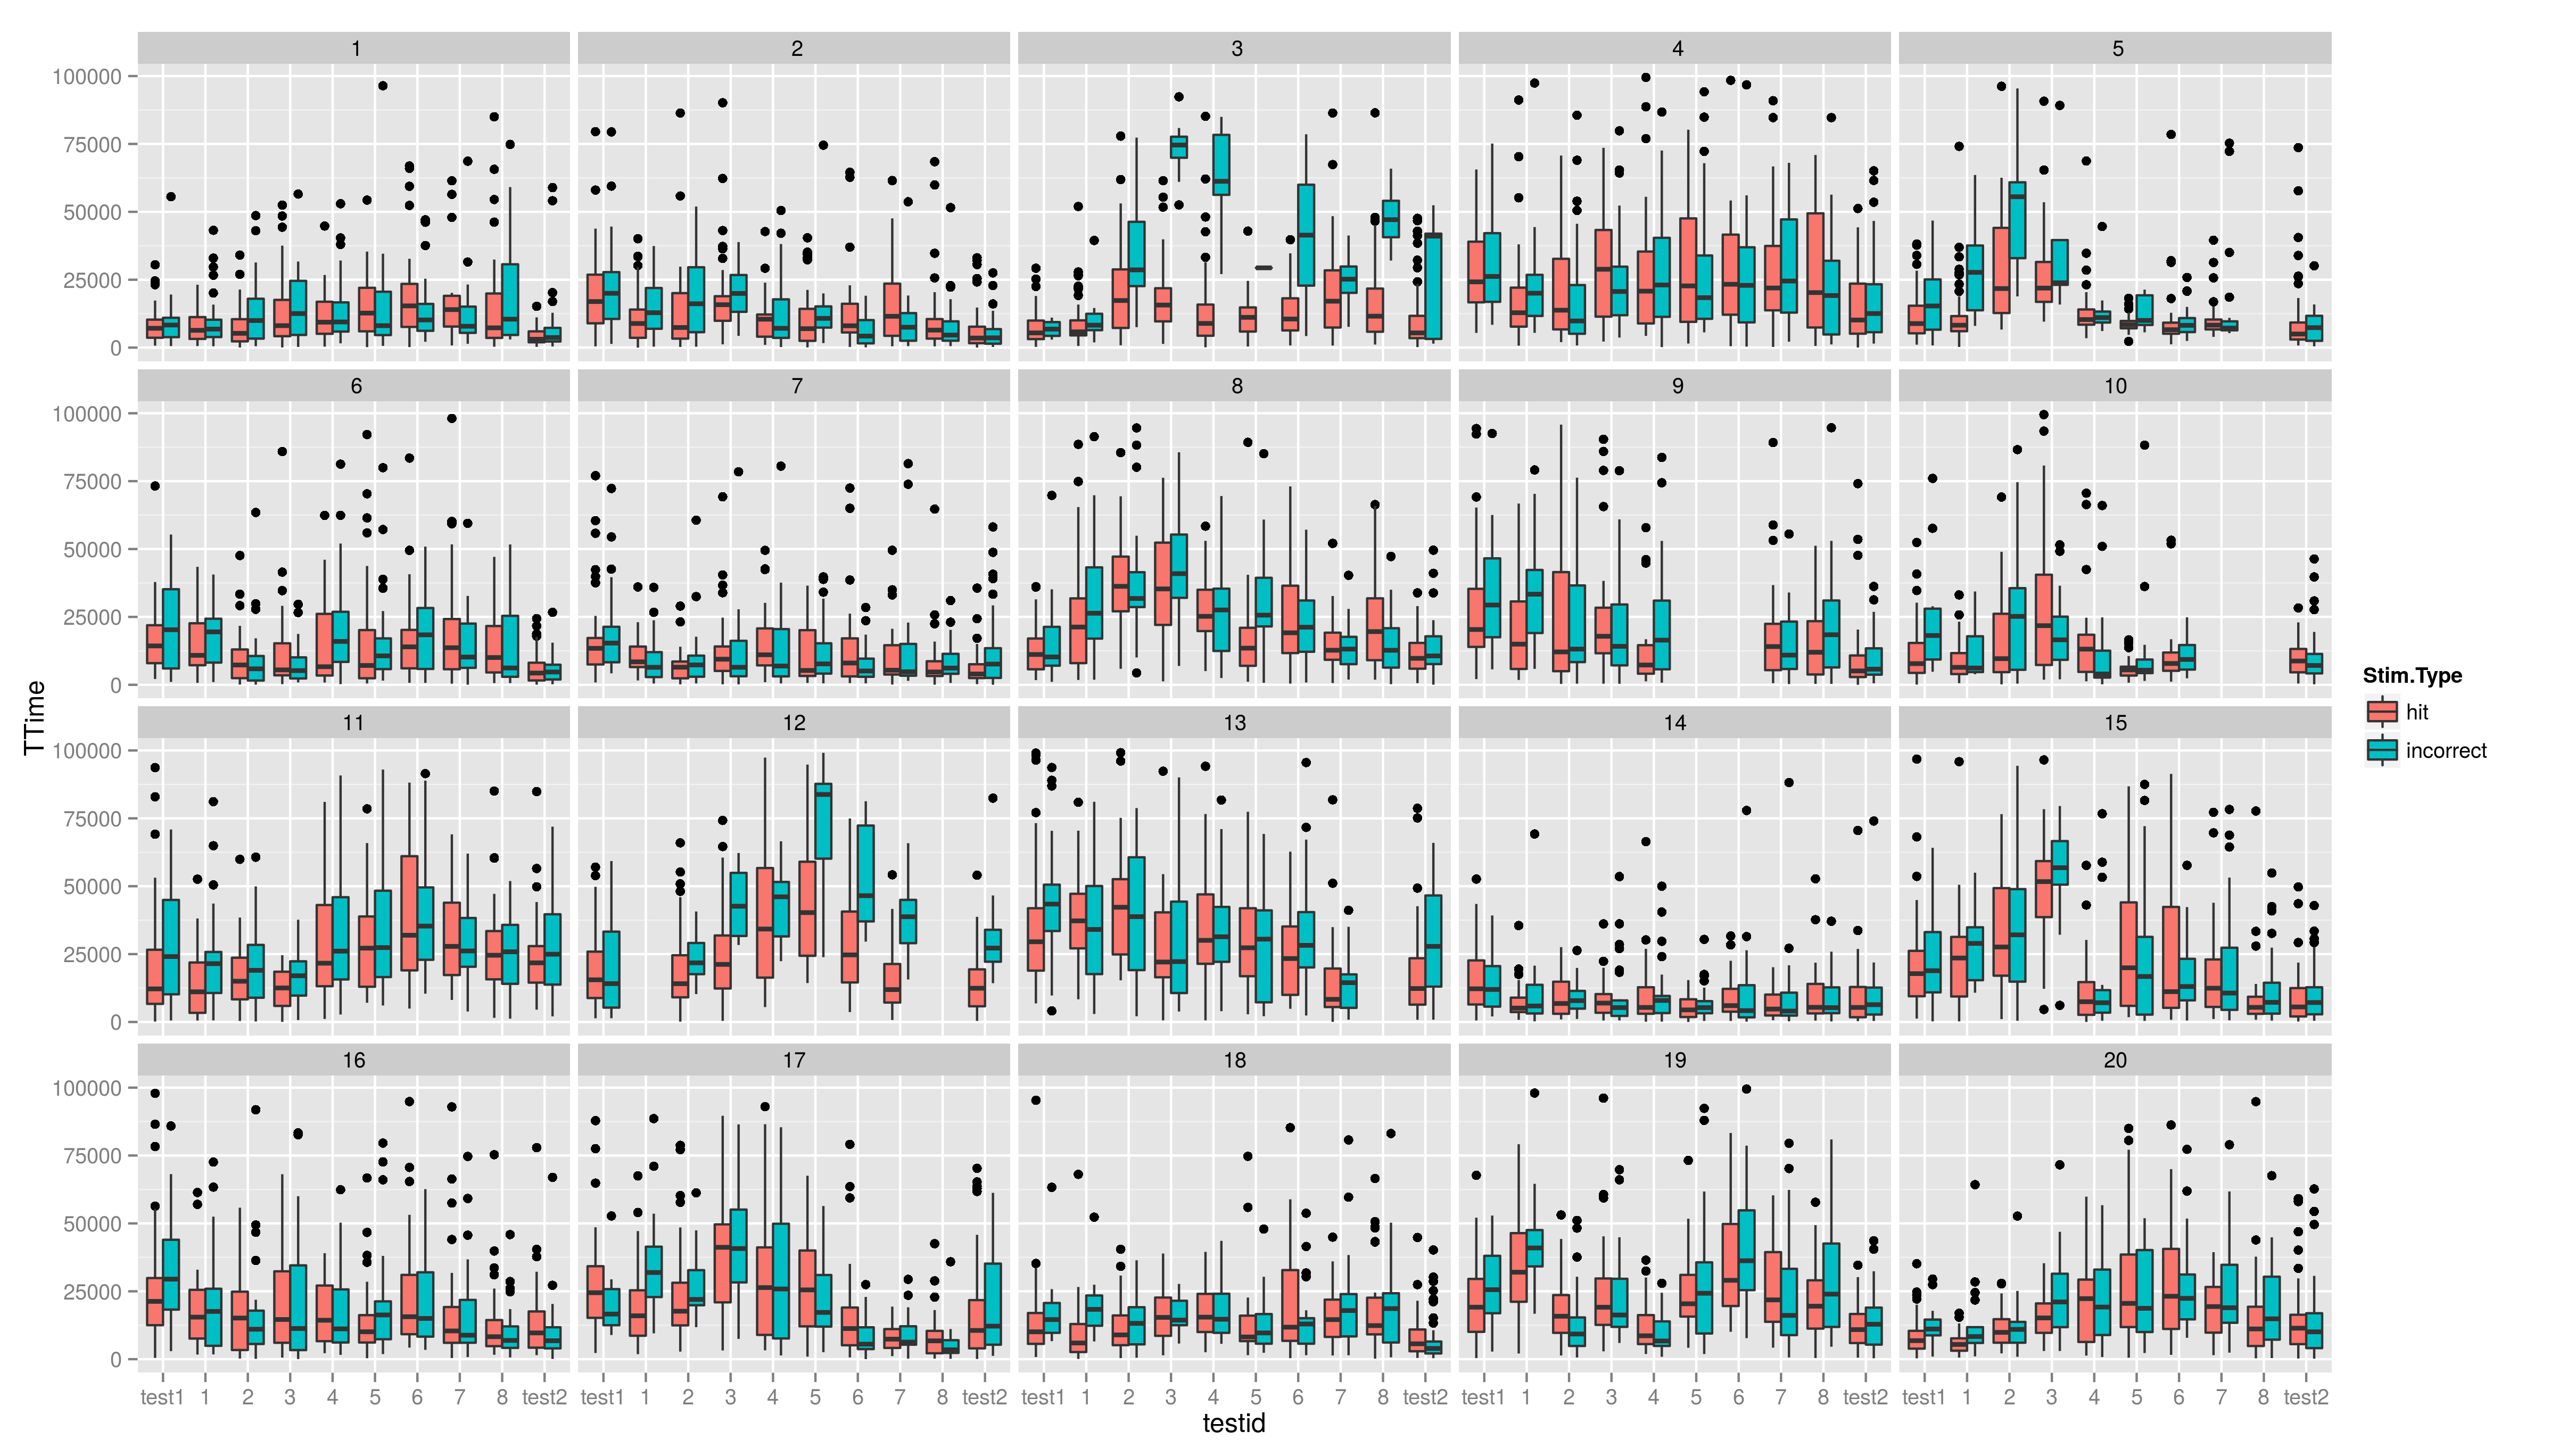
\includegraphics[width=10cm]{boxplotfacets.png}
\end{center}
\end{frame}


